\documentclass[a4paper,12pt]{article}
\usepackage{ragged2e}
\usepackage{graphicx}
\usepackage{float}
\usepackage{mathtools}
\usepackage{amsmath}
\usepackage[utf8]{inputenc}

\begin{document}
\begin{titlepage}
	\vspace*{\stretch{1.0}}
		\begin{center}
			\large\textbf{Proyecto Final}\\
			\large\textit{Brian de Jesus Herberth Guerrero}\\
			\large\textit{A00398663}
		\end{center}
	\vspace*{\stretch{2.0}}
\end{titlepage}

\section{Del siguiente tutorial, capturar y documentar en latex los ejercicios}
https://www.gnu.org/software/octave/doc/v4.0.0/Simple-Examples.html

\subsection{Elementary calculations}
\justifying
\par
Octave can easily be used for basic numerical calculations. Octave knows about arithmetic operations(+,-,*,/), exponentiation, natural logarithms / exponents (log, exp), and the trigonometric functions (sin, cos, …). Moreover, Octave calculations work on real or imaginary numbers (i,j). In addition, some mathematical constants such as the base of the natural logarithm (e) and the ratio of a circle’s circumference to its diameter (pi) are pre-defined.
\par
For example, to verify Euler’s Identity,
\begin{equation}
    \label{simple_equation}
    i * pi
\end{equation}
\begin{equation}
    \label{simple_equation}
    e = -1
\end{equation}
\par
type the following which will evaluate to -1 within the tolerance of the calculation.
\begin{equation}
    \label{simple_equation}
    octave:1> exp (i*pi)
\end{equation}
\par
Here is an image which shows the program execution
\begin{figure}[H]
    \centering
    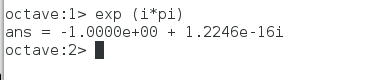
\includegraphics[width=3.0in]{img/1.png}
    \caption{Elementary calculations}
    \label{simulationfigure}
\end{figure}

\subsection{Creating a matrix}
\justifying
\par
Vectors and matrices are the basic building blocks for numerical analysis. To create a new matrix and store it in a variable so that you can refer to it later, type the command
\begin{equation}
    \label{simple_equation}
    octave:1> A = [ 1, 1, 2; 3, 5, 8; 13, 21, 34 ]
\end{equation}
\par
Octave will respond by printing the matrix in neatly aligned columns. Octave uses a comma or space to separate entries in a row, and a semicolon or carriage return to separate one row from the next. Ending a command with a semicolon tells Octave not to print the result of the command. For example,
\begin{equation}
    \label{simple_equation}
    octave:2> B = rand (3, 2);
\end{equation}
\par
will create a 3 row, 2 column matrix with each element set to a random value between zero and one.
\par
To display the value of a variable, simply type the name of the variable at the prompt. For example, to display the value stored in the matrix B, type the command
\begin{equation}
    \label{simple_equation}
    octave:3> B
\end{equation}
\par
Here is an image which shows the program execution
\begin{figure}[H]
    \centering
    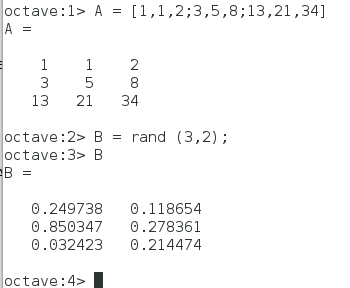
\includegraphics[width=3.0in]{img/2.png}
    \caption{Creating a Matrix}
    \label{simulationfigure}
\end{figure}

\subsection{Matrix arithmetic}
\justifying
\par
Octave has a convenient operator notation for performing matrix arithmetic. For example, to multiply the matrix A by a scalar value, type the command
\begin{equation}
    \label{simple_equation}
	octave:4> 2 * A
\end{equation}
\par
To multiply the two matrices A and B, type the command
\begin{equation}
    \label{simple_equation}
	octave:5> A * B
\end{equation}
\par
and to form the matrix product transpose (A) * A, type the command
\begin{equation}
    \label{simple_equation}
	octave:6> A' * A
\end{equation}
\par
Here is an image which shows the program execution
\begin{figure}[H]
    \centering
    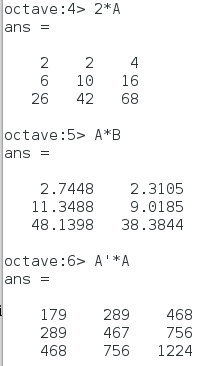
\includegraphics[width=3.0in]{img/3.png}
    \caption{Matrix arithmetic}
    \label{simulationfigure}
\end{figure}

\subsection{Solving systems of linear equations}
\justifying
\par
Systems of linear equations are ubiquitous in numerical analysis. To solve the set of linear equations Ax = b, use the left division operator, ‘\textbackslash’:
\begin{equation}
    \label{simple_equation}
	x = A \ b
\end{equation}
\par
This is conceptually equivalent to inv (a) * b, but avoids computing the inverse of a matrix directly.
\par
If the coefficient matrix is singular, Octave will print a warning message and compute a minimum norm solution.
\par
A simple example comes from chemistry and the need to obtain balanced chemical equations. Consider the burning of hydrogen and oxygen to produce water.
\begin{equation}
    \label{simple_equation}
	H2 + O2 --> H2O
\end{equation}
\par
The equation above is not accurate. The Law of Conservation of Mass requires that the number of molecules of each type balance on the left- and right-hand sides of the equation. Writing the variable overall reaction with individual equations for hydrogen and oxygen one finds:

\begin{equation}
    \label{simple_equation}
	x1*H2 + x2*O2 --> H2O
\end{equation}
\begin{equation}
    \label{simple_equation}
	H: 2*x1 + 0*x2 --> 2
\end{equation}
\begin{equation}
    \label{simple_equation}
	O: 0*x1 + 2*x2 --> 1
\end{equation}
\par
The solution in Octave is found in just three steps.

\begin{equation}
    \label{simple_equation}
	octave:1> A = [ 2, 0; 0, 2 ];
\end{equation}
\begin{equation}
    \label{simple_equation}
	octave:2> b = [ 2; 1 ];
\end{equation}
\begin{equation}
    \label{simple_equation}
	octave:3> x = A \ b
\end{equation}

\par
Here is an image which shows the program execution
\begin{figure}[H]
    \centering
    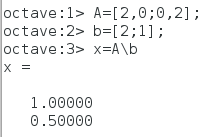
\includegraphics[width=3.0in]{img/4.png}
    \caption{Solving systems of linear equations}
    \label{simulationfigure}
\end{figure}

\subsection{Integrating differential equations}
\justifying
\par
Octave has built-in functions for solving nonlinear differential equations of the form
\begin{equation}
    \label{simple_equation}
	dx/dt = f (x, t)	
\end{equation}
\par
with the initial condition
\begin{equation}
    \label{simple_equation}
	x(t = t0) = x0
\end{equation}
\par
For Octave to integrate equations of this form, you must first provide a definition of the function f(x,t). This is straightforward, and may be accomplished by entering the function body directly on the command line. For example, the following commands define the right-hand side function for an interesting pair of nonlinear differential equations. Note that while you are entering a function, Octave responds with a different prompt, to indicate that it is waiting for you to complete your input.
\begin{flushleft}
	octave:1\textgreater function xdot = f (x, t)\\
	\textgreater\\
	\textgreater  r = 0.25;\\
	\textgreater  k = 1.4;\\
	\textgreater  a = 1.5;\\
	\textgreater  b = 0.16;\\
	\textgreater  c = 0.9;\\
	\textgreater  d = 0.8;\\
	\textgreater \\
	\textgreater  xdot(1) = r*x(1)*(1 - x(1)/k) - a*x(1)*x(2)/(1 + b*x(1));\\
	\textgreater  xdot(2) = c*a*x(1)*x(2)/(1 + b*x(1)) - d*x(2);\\
	\textgreater \\
	\textgreater endfunction\\
\end{flushleft}
\par
	Given the initial condition
\begin{equation}
    \label{simple_equation}
	octave:2> x0 = [1; 2];
\end{equation}
\par
and the set of output times as a column vector (note that the first output time corresponds to the initial condition given above)
\begin{equation}
    \label{simple_equation}
	octave:3> t = linspace (0, 50, 200)';
\end{equation}
\par
it is easy to integrate the set of differential equations:
\begin{equation}
    \label{simple_equation}
	octave:4> x = lsode ("f", x0, t);
\end{equation}
\par
The function lsode uses the Livermore Solver for Ordinary Differential Equations, described in A. C. Hindmarsh, ODEPACK, a Systematized Collection of ODE Solvers, in: Scientific Computing, R. S. Stepleman et al. (Eds.), North-Holland, Amsterdam, 1983, pages 55–64.
\par
Here is an image which shows the program execution
\begin{figure}[H]
    \centering
    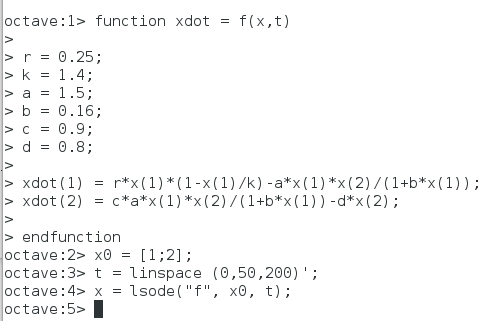
\includegraphics[width=3.0in]{img/5.png}
    \caption{Integrating differential equations}
    \label{simulationfigure}
\end{figure}

\subsection{Producing graphical output}
\justifying
\par
To display the solution of the previous example graphically, use the command
\begin{equation}
    \label{simple_equation}
	octave:1> plot (t, x)
\end{equation}
\par
If you are using a graphical user interface, Octave will automatically create a separate window to display the plot.
\par
To save a plot once it has been displayed on the screen, use the print command. For example,
\begin{equation}
    \label{simple_equation}
	print -dpdf foo.pdf
\end{equation}
\par
will create a file called foo.pdf that contains a rendering of the current plot in Portable Document Format. The command
\begin{equation}
    \label{simple_equation}
	help print
\end{equation}
\par
explains more options for the print command and provides a list of additional output file formats.
\par
Here is an image which shows the program execution
\begin{figure}[H]
    \centering
    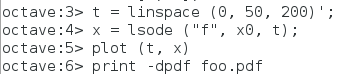
\includegraphics[width=3.0in]{img/6.png}
    \caption{Creating plot}
    \label{simulationfigure}
\end{figure}
\par
Here is an image of the Plot
\begin{figure}[H]
    \centering
    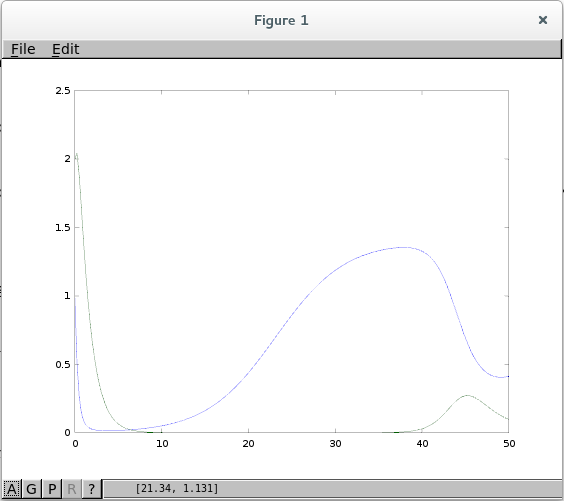
\includegraphics[width=3.0in]{img/7.png}
    \caption{Plot}
    \label{simulationfigure}
\end{figure}

\section{Proyecto de clase}
\justifying
\par
Resolver nuevamente el proyecto de clase, pero cambiar el conjunto de datos del archivo .txt, con al menos 200 renglones de algun tema en especial de su interes (salud, sismos, peliculas, musica, videos).
\par
Well, I searched for data about earthquakes, this data is about the earthquakes in the last two weeks\\ 
First, we'll want to load the data:
\begin{equation}
    \label{simple_equation}
	data = load('txt/sismos.txt');
\end{equation}
\par
Next, let's define x and y. The x vector is for the independent variable (the number of earthquakes), and the y vector is for the dependent variable (magnitude of earthquakes). 
\begin{equation}
    \label{simple_equation}
	x = data(:,1);
\end{equation}
\begin{equation}
    \label{simple_equation}
	y = data(:,2);
\end{equation}
\par
Let's create a function to plot the data
\begin{equation}
    \label{simple_equation}
	function plotData(x,y)
\end{equation}
\begin{equation}
    \label{simple_equation}
	plot(x,y,'rx','MarkerSize',2);
\end{equation}
\begin{equation}
    \label{simple_equation}
	end
\end{equation}
\begin{equation}
    \label{simple_equation}
	plotData(x,y);
\end{equation}
\begin{equation}
    \label{simple_equation}
	xlabel('Number of earthquakes');
\end{equation}
\begin{equation}
    \label{simple_equation}
	ylabel('magnitude of earthquakes');
\end{equation}
\begin{equation}
    \label{simple_equation}
	fprintf('Program paused. Press enter to continue.');
\end{equation}
\begin{equation}
    \label{simple_equation}
	pause;
\end{equation}
\par
 And the graph of the data looks like this:
\begin{figure}[H]
    \centering
    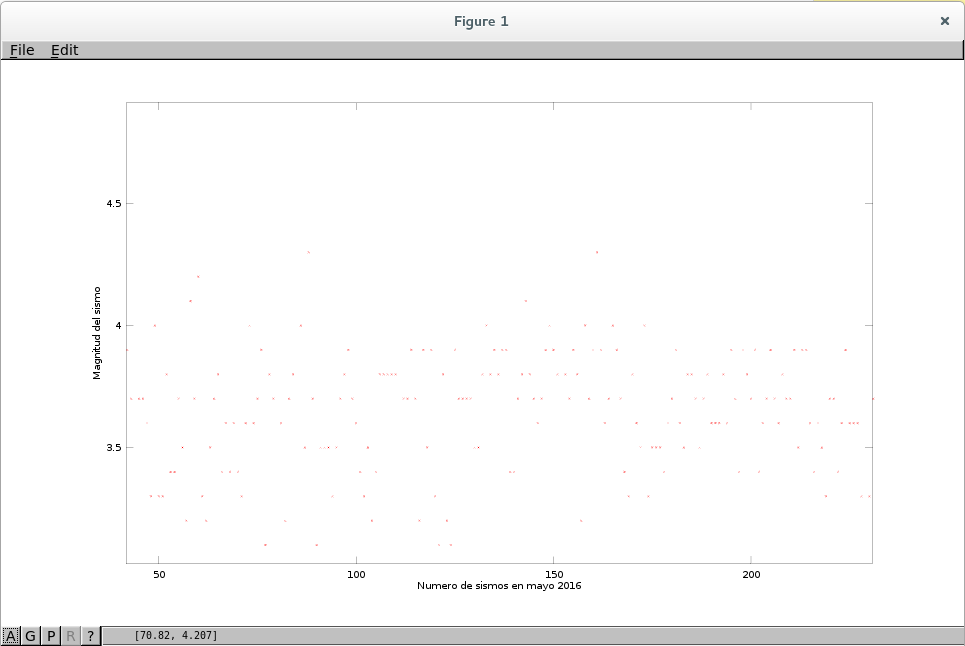
\includegraphics[width=3.0in]{img/8.png}
    \caption{Plot of earthquakes}
    \label{simulationfigure}
\end{figure}
\par
Add a column of all ones to our x column
\begin{equation}
    \label{simple_equation}
	m = length(x);
\end{equation}
\begin{equation}
    \label{simple_equation}
	X = [ones(m, 1) x];
\end{equation}
\par
Now use the normal equation to calculate theta. Basically, we are minimizing the sum of the squared errors between our predicted equation and the actual y values. 
\begin{equation}
    \label{simple_equation}
	Theta = (X exp(T) X)exp(negativo(1)) X exp(T)y
\end{equation}
\par
Putting that into Octave:
\begin{equation}
    \label{simple_equation}
	Theta = (X exp(T) X)exp(negativo(1)) X exp(T)y
\end{equation}
\par
\begin{equation}
    \label{simple_equation}
	theta = (pinv(X'*X))*X'*y
\end{equation}
\begin{equation}
    \label{simple_equation}
	theta = 3.6026e+00
\end{equation}
\begin{equation}
    \label{simple_equation}
	theta = 2.5022e-04
\end{equation}
\par
Now, let's plot our fitted equation (prediction) on top of the training data, to see if our fitted equation makes sense.
\begin{equation}
    \label{simple_equation}
	hold on; 
\end{equation}
\begin{equation}
    \label{simple_equation}
	plot(X(:,2), X*theta, -)
\end{equation}
\begin{equation}
    \label{simple_equation}
	legend('Training data', Linear regression)
\end{equation}
\begin{equation}
    \label{simple_equation}
	hold off
\end{equation}
And the graph of the data looks like this:
\begin{figure}[H]
    \centering
    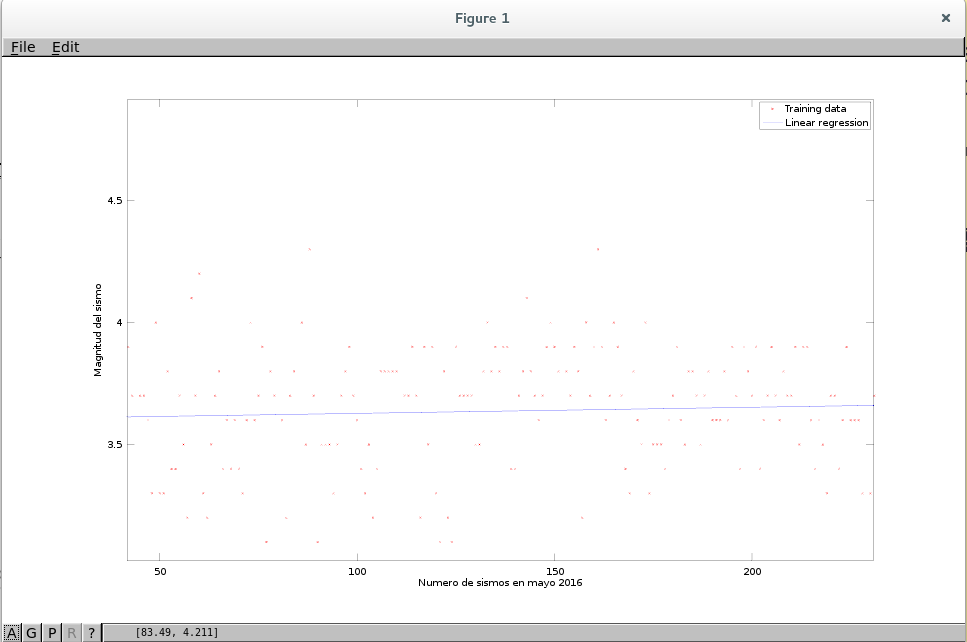
\includegraphics[width=3.0in]{img/9.png}
    \caption{prediction}
    \label{simulationfigure}
\end{figure}
Here is an image which shows the program execution
\begin{figure}[H]
    \centering
    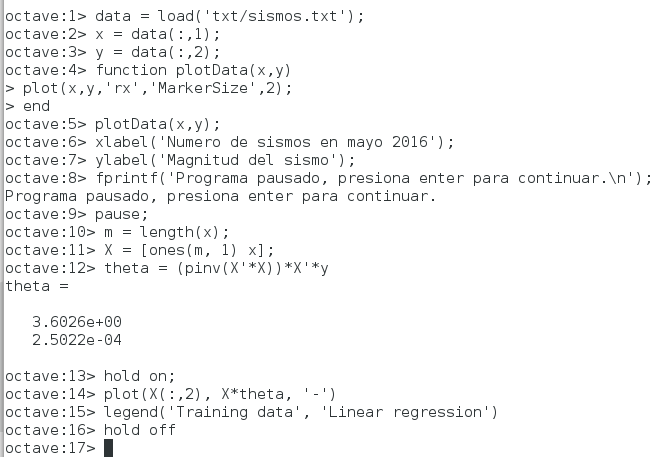
\includegraphics[width=3.0in]{img/10.png}
    \caption{Program execution}
    \label{simulationfigure}
\end{figure}

\section{Lectura del articulo: Deep Learning}
\justifying
\par
http://www.xataka.com/robotica-e-ia/deep-learning-que-es-y-por-que-va-a-ser-una-tecnologia-clave-en-el-futuro-de-la-inteligencia-artificial
\par
Desde los años 50 del siglo pasado y hasta hace muy pocos años el terreno habitual de la Inteligencia Artificial avanzada era mayoritariamente el laboratorio de investigación y la ciencia ficción.
\par
El gran impulso tecnológico al que solemos referirnos bajo el término Big Data ha revolucionado el entorno empresarial. Las organizaciones sometidas a la necesidad de la transformación digital se han convertido en criaturas sedientas de cantidades ingentes de datos; y por primera vez en la historia de la IA existe una demanda generalizada de sistemas con una inteligencia avanzada, equivalente a la de un humano, que sean capaces de procesar esos datos.
\par
Una de las claves de la IA avanzada está en el aprendizaje. Es cada vez más habitual que les pidamos a las máquinas que aprendan por sí solas, por lo cual necesitamos que las máquinas sean capaces de auto-programarse, en otras palabras, queremos máquinas que aprendan de su propia experiencia. La disciplina del Aprendizaje Automático (Machine Learning)
\par
En el enfoque Deep Learning se usan estructuras lógicas que se asemejan en mayor medida a la organización del sistema nervioso de los mamíferos, teniendo capas de unidades de proceso (neuronas artificiales) que se especializan en detectar determinadas características existentes en los objetos percibidos. La visión artificial es una de las áreas donde el Deep Learning proporciona una mejora considerable en comparación con algoritmos más tradicionales. Existen varios entornos y bibliotecas de código de Deep Learning que se ejecutan en las potentes GPUs modernas tipo CUDA, como por ejemplo NVIDIA cuDNN.
\par
Los modelos computacionales de Deep Learning imitan estas características arquitecturales del sistema nervioso, permitiendo que dentro del sistema global haya redes de unidades de proceso que se especialicen en la detección de determinadas características ocultas en los datos. Este enfoque ha permitido mejores resultados en tareas de percepción computacional, si las comparamos con las redes monolíticas de neuronas artificiales.
\par
El internet de las cosas (IoT) supone un gran avance en el reto de la adquisición de los datos, mientras que la computación cognitiva aporta la inteligencia necesaria para la extracción del conocimiento.
\par
La Internet Cognitiva y Ubicua cuenta con un sistema sensorial que no para de extenderse gracias a los miles de millones de sensores conectados y desplegados por todas partes.
\par
El auge de los sistemas M2M (Machine to Machine) en el marco del Internet de las Cosas ha promovido un crecimiento exponencial del intercambio de datos entre las propias máquinas.
\par
Con la llegada de tecnologías como el Deep Learning y la Computación Cognitiva nuestra forma de aprender, de relacionarnos y de entender el mundo va a cambiar también de forma radical.
\par
\textbf{Dr. Raúl Arrabales Moreno}

\section{Resumen}
\justifying
\par
Realizar un resumen de 1 cuartilla del tema que consideren de mayor interes para su carrera profesional\\
\par
\textbf{La Ingeniería Mecatrónica, una carrera del futuro que se vive desde hoy}\\
\par
Muchas personas piensan que el ingeniero mecatrónico pasa su vida en la creación de robots sin ninguna utilidad práctica inmediata. Pero la presencia de un profesional de este campo es mucho más importante de lo que crees.\\
\par
Las labores de un ingeniero mecatronico incluyen:
\begin{itemize}
\item Implementar sistemas inteligentes, usando la electrónica moderna y la tecnología de los materiales
\item Realizar la automatización y el control de procesos, integrando sistemas con sensores, actuadores e interfases hombre-máquina
\item Armar y coordinar equipos de trabajo para realizar proyectos mecatrónicos
\item Diseñar e implementar sistemas roboticos
\end{itemize}
\par
Al igual que la industria aeroespacial, la mayoría de las cosas que necesitamos hoy en día dependen de equipos, máquinas y sistemas mecatrónicos. El ingeniero mecatrónico es responsable de reunir los conocimientos especializados en Mecánica, Electrónica e Informática con el fin de desarrollar la mejor solución a las actividades humanas.\\
\par
Al igual que en cualquier otra ingeniería, es importante tener una buena capacidad de abstracción y la facilidad para trabajar en equipo. Debido a que es una profesión que interconecta otras disciplinas, la Ingeniería Mecatrónica requiere paciencia y comunicabilidad.\\
\par
El papel de los profesionales se centra principalmente en la industria manufacturera. Esto incluye las plantas de energía, fábricas de acero, plantas de automóviles y medicamentos, entre otros. El mundo actual obliga a ser interdisciplinario, conocer la Ingeniería de control y automatización para que gracias a ellos los procesos sean óptimos.\\
\par
La Ingeniería Mecatrónica integra los conocimientos, procedimientos y tecnologías provenientes de la ingeniería mecánica, electrónica, informática y eléctrica. Esta sinergia permite el análisis, diseño de productos y procesos de manufacturas automatizadas.\\
\par
La UTP forma profesionales altamente calificados en la automatización de sistemas de producción industrial y de manufacturas, utilizando técnicas electrónicas e informáticas de última generación.\\
\par
Es una carrera con gran futuro, puesto que la tendencia mundial es que las máquinas reemplacen el trabajo manual con lo cual los profesionales de esta carrera serán los más requeridos.\\
\par

\end{document}